\documentclass[t,aspectratio=169]{beamer}
\usetheme[progressbar=frametitle]{metropolis}
\usefonttheme{professionalfonts}
\usepackage{appendixnumberbeamer}

\usepackage{booktabs}
\usepackage[scale=2]{ccicons}

\usepackage{graphics,graphicx,amssymb,amsmath,pgf,comment,hyperref}
%\usepackage[xcolor=pst]{pstricks}
\usepackage{array}
\usepackage{pgfshade}
\usepackage[round]{natbib}
\usepackage[absolute,overlay]{textpos}
\usepackage{pifont}
\usepackage{dcolumn}
\usepackage{textpos}
\usepackage{color}					
\usepackage{xcolor,colortbl}
\usepackage{tikz}
\usepackage{bbm}
\usepackage{curves}
\usepackage{mathtools}
\usepackage{times}
\usepackage{verbatim}
\usetikzlibrary{snakes,arrows,shapes,positioning}
\def\augie{\fontencoding{T1}\fontfamily{augie}\selectfont}

\usepackage{pgfplots}
\usepgfplotslibrary{dateplot}

\usepackage{xspace}
\newcommand{\themename}{\textbf{\textsc{metropolis}}\xspace}

\setbeamertemplate{caption}{\raggedright\insertcaption\par}
\usetikzlibrary{calc,decorations.pathmorphing,patterns}
\pgfdeclaredecoration{penciline}{initial}{
    \state{initial}[width=+\pgfdecoratedinputsegmentremainingdistance,
    auto corner on length=1mm,]{
        \pgfpathcurveto%
        {% From
            \pgfqpoint{\pgfdecoratedinputsegmentremainingdistance}
                      {\pgfdecorationsegmentamplitude}
        }
        {%  Control 1
        \pgfmathrand
        \pgfpointadd{\pgfqpoint{\pgfdecoratedinputsegmentremainingdistance}{0pt}}
                    {\pgfqpoint{-\pgfdecorationsegmentaspect
                     \pgfdecoratedinputsegmentremainingdistance}%
                               {\pgfmathresult\pgfdecorationsegmentamplitude}
                    }
        }
        {%TO
        \pgfpointadd{\pgfpointdecoratedinputsegmentlast}{\pgfpoint{1pt}{1pt}}
        }
    }
    \state{final}{}
}


\title{Owning the Agent: Hospital Influence on Physician Behaviors}
\date{}
\author{Haizhen Lin \& \textbf{Ian McCarthy} \& Michael Richards}
\institute{September 6, 2019}

\begin{document}
\tikzstyle{every picture}+=[remember picture]
\everymath{\displaystyle}

\maketitle

\section{Background}

\begin{frame}{Physician Agency}
    \only<1>{
        Physician with decision-making authority for treatment
        \begin{itemize}
            \item Information asymmetry
            \item Regulatory restrictions
        \end{itemize}
    }
    \only<2->{
        Differential financial incentives between physician and hospital
        \begin{itemize}
            \item More procedures $=$ more revenue, but location of procedure may matter to hospital
            \item Hospital wants less cost with fixed payment, but physician dictates resource use
            \item Hospital as residual claimant on billable physician services
        \end{itemize}
    }
    \onslide<3->{
        $\longrightarrow$ Incentives for hospitals to influence physicians \\
        \vspace{.25in}
    }
    \onslide<4->{
        \noindent Most direct way (arguably) is to purchase physician practice
    }
\end{frame}

\begin{frame}{Changing Physician Relationships}
    \only<1>{
        \begin{figure}
            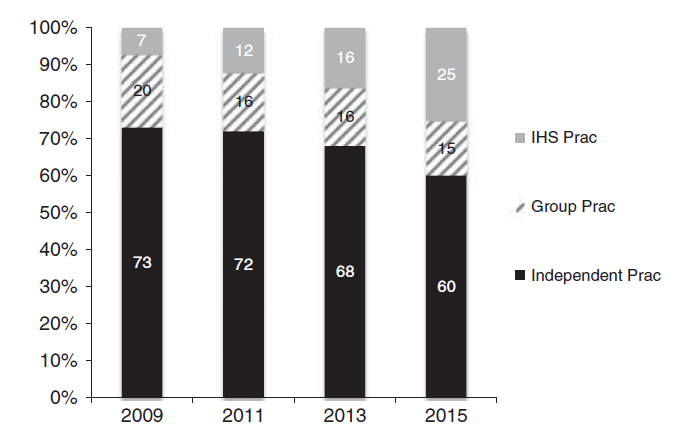
\includegraphics[height=2.4in,keepaspectratio]{Richardsetal.png}
            \caption{Richards \textit{et al.}, Medical Care, 2016}
        \end{figure}
    }
    \only<2>{
        \begin{figure}
            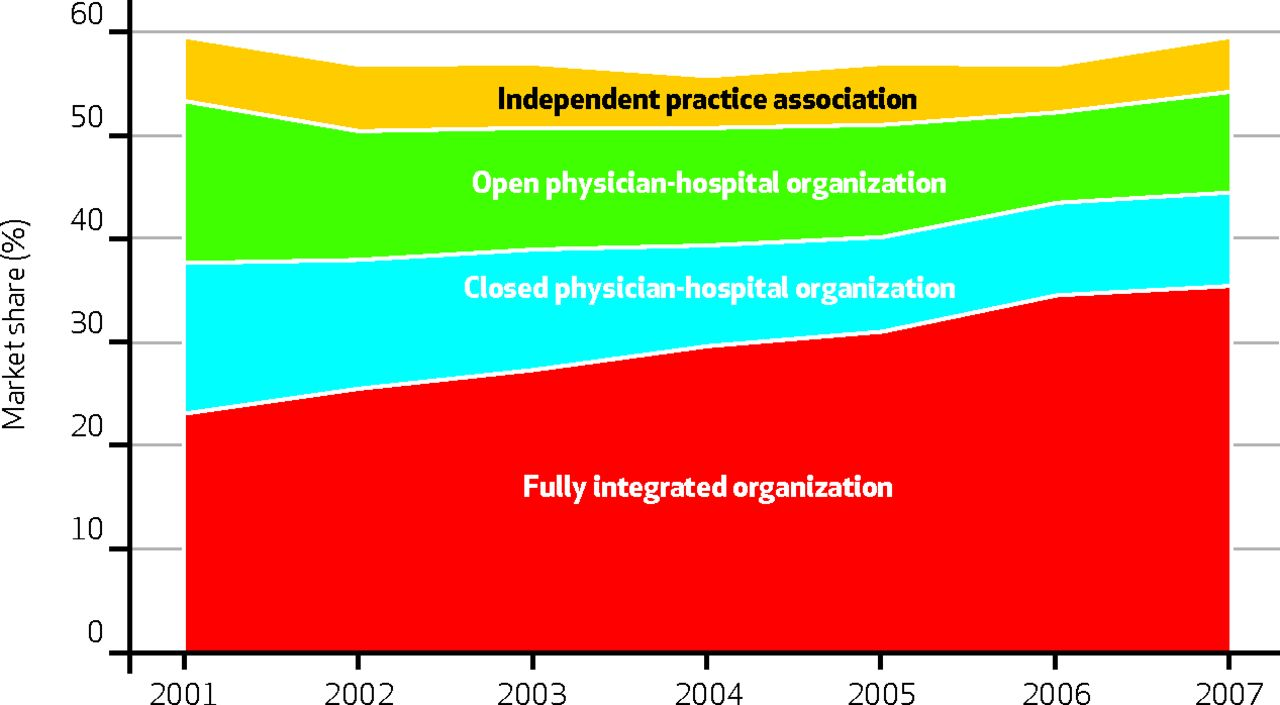
\includegraphics[height=2.3in,keepaspectratio]{Bakeretal.jpg}
            \caption{Baker, Bundorf, and Kessler, Health Affairs, 2014}
        \end{figure}
    }
\end{frame}

\begin{frame}{In context}
    \begin{itemize}
        \item Physician agency (Clemens \& Gottlieb 2014, AER; Afendulis \& Kessler 2007, AER; Gruber \& Owings 1996, RAND; Iizuka 2012, AER)
        \item Supply-side variation (Finkelstein \textit{et al.} 2016, QJE; Molitor 2018, AEJ: Policy)
        \item Vertical integration (Cuellar \& Gertler 2006, JHE; Ciliberto \& Dranove 2006, JHE; Baker \textit{et al.} 2016, JHE; Koch \textit{et al.} 2017, JHE)
    \end{itemize}
\end{frame}

\begin{frame}{Outline}
    \begin{enumerate}
        \item Conceptual Framework
        \item Initial Results
        \item Event Study
        \item Instrumental Variables
        \item Other Outcomes
    \end{enumerate}
\end{frame}

\section{Conceptual Framework}
\begin{frame}{Physician Agency}
    \tikzstyle{na} = [baseline=-.5ex]
    \only<1->{
        Observed care at time $t$ is
        \begin{equation*}
            y_{ijk} = \arg \max_{y}  \theta_{u} \tilde{u} \left(y; \Gamma_{k}, \Gamma_{j}, \kappa_{i} \right) + \theta_{\pi} \pi \left(y; \Gamma_{k}, \Gamma_{j}, \kappa_{i} \right).
        \end{equation*}
    }
    \only<2->{
        \noindent With assumptions on linearity and separability in patient preferences:
        \begin{equation*}
            y_{ijk} =
            \tikz[baseline]{
                \node[fill=blue!20,anchor=base] (t1)
                {$ \alpha_{i} + x_{i}\beta $};
            } +
            \tikz[baseline]{
                \node[fill=red!20, ellipse, anchor=base] (t2)
                {$\Gamma_{jk}$};
            } + \epsilon_{ijk}
        \end{equation*}
        \begin{itemize}[<+-| alert@+>]
            \item[]<3-> Patient Preferences
                \tikz[na] \node[coordinate] (n1) {};
            \item[]<4-> Physician and hospital characteristics
                \tikz[na] \node[coordinate] (n2) {};
        \end{itemize}

        \begin{tikzpicture}[overlay]
            \path[->]<3-> (n1) edge [bend right] (t1);
            \path[->]<4-> (n2) edge [out=0, in=-90] (t2);
        \end{tikzpicture}
    }
\end{frame}

\begin{frame}{Estimation Strategy}
    \tikzstyle{na} = [baseline=-.5ex]
    \only<1-3>{
        Suggests two-step estimation strategy:
        \begin{enumerate}
            \item<2-> Estimate $y_{ijk} = \alpha_{i} + x_{i}\beta + \Gamma_{jk} + \epsilon_{ijk}$ at patient level (separately by year). This isolates variation in care to physicians and hospitals (not patients).
            \item<3-> Estimate $\hat{\Gamma}_{jkt} = \gamma_{j} + \gamma_{k} + \tau_{t} + z_{jkt}\delta + \eta_{jkt}$ with physician-hospital panel. This further isolates variation to physician-hospital interaction.
        \end{enumerate}
    }
    \only<4>{
        \begin{itemize}
            \item Draws from ``match values'' in labor literature (Abowd \textit{et al.}, 2002; Card \textit{et al.}, 2013, QJE )
            \item Exploits variation across inpatient stays and splits the separation of match value into two steps
            \item Identifies effects on match value from within-physician variation across hospitals (e.g., patient movers in Finkelstein \textit{et al.}, 2016, QJE)
        \end{itemize}
    }
    \only<5-8>{
        Traditional ``match value'' approach:
        \begin{equation*}
            y_{ijk} = \alpha_{i} + x_{i}\beta +
            \tikz[baseline]{
                \node[fill=blue!20,anchor=base] (t1)
                {$\Gamma_{j}$};
            } +
            \tikz[baseline]{
                \node[fill=green!20,anchor=base] (t2)
                {$\Gamma_{k}$};
            } +
            \tikz[baseline]{
                \node[fill=red!20,ellipse,anchor=base] (t3)
                {$\Gamma_{jk}$};
            } +
            \epsilon_{ijk}
        \end{equation*}
        \begin{itemize}[<+-| alert@+>]
            \item[]<6-> Physician effect
                \tikz[na] \node[coordinate] (n1) {};
            \item[]<7-> Hospital effect
                \tikz[na] \node[coordinate] (n2) {};
            \item[]<8-> Physician-hospital match value
                \tikz[na] \node[coordinate] (n3) {};
        \end{itemize}

        \begin{tikzpicture}[overlay]
            \path[->]<6-> (n1) edge [bend right] (t1);
            \path[->]<7-> (n2) edge [out=10, in=-70] (t2);
            \path[->]<8-> (n3) edge [out=0, in=-90] (t3);
        \end{tikzpicture}
    }
    \only<9->{
        Our approach:
        \begin{equation*}
            y_{ijk} = \alpha_{i} + x_{i}\beta + \underbrace{
            \tikz[baseline]{
                \node[fill=blue!20,anchor=base] (t1)
                {$\Gamma_{jk}^{t}$};
            }}_{
            \tikz[baseline]{
                \node[fill=green!20,anchor=base] (t2)
                {$\Gamma_{j}$};
            } +
            \tikz[baseline]{
                \node[fill=red!20,anchor=base] (t3)
                {$\Gamma_{k}$};
            } +
            \tikz[baseline]{
                \node[fill=orange!20,ellipse,anchor=base] (t4)
                {$z_{jkt}\delta$};
            }} +
            \epsilon_{ijk}
        \end{equation*}
        \begin{itemize}[<+-| alert@+>]
            \item[]<10-> Physician, hospital, and match effect (jointly)
                \tikz[na] \node[coordinate] (n1) {};
            \item[]<11-> Physician effect
                \tikz[na] \node[coordinate] (n2) {};
            \item[]<12-> Hospital effect
                \tikz[na] \node[coordinate] (n3) {};
            \item[]<13-> Physician-hospital integration
                \tikz[na] \node[coordinate] (n4) {};
        \end{itemize}

        \begin{tikzpicture}[overlay]
            \path[->]<10-> (n1) edge [out=0, in=-90] (t1);
            \path[->]<11-> (n2) edge [out=10, in=-70] (t2);
            \path[->]<12-> (n3) edge [out=5, in=-80] (t3);
            \path[->]<13-> (n4) edge [out=0, in=-90] (t4);
        \end{tikzpicture}
    }
\end{frame}

\begin{frame}{Intuition}
    \begin{itemize}
        \item Hospital influence on physicians is an interaction effect
        \item Potential influence should be net of patient preference
        \item Why not estimate in single step?
        \begin{itemize}
            \item Treatment assignment should be at physician/hospital level
            \item Weights by number of patients
            \item Computationally infeasible with same specification
        \end{itemize}
    \end{itemize}
\end{frame}

\section{Data}
\begin{frame}{Data Sources}
    \begin{itemize}
        \item CMS: 100\% inpatient and institutional outpatient Medicare claims data (2008-2015)
        \item SK\&A: Hospital ownership of physician practices and practice characteristics
        \item AHA, HCRIS, POS: Hospital characteristics
        \item Annual IPPS Impact Files: Hospital cost-to-charge ratios (CCR)
        \item ACS: County-level demographics, education, income, and employment
    \end{itemize}
\end{frame}

\begin{frame}{Sample Construction}
    \begin{itemize}
        \item<1-> Planned inpatient stays (elective admissions initiated by a physician, clinic, or HMO referral) and outpatient procedures with observed NPI for the operating physician
        \item<2-> Drop physicians operating in hospitals more than 120 miles from primary office or outside of contiguous U.S.
        \item<3-> Drop physicians with NPIs not matched in the SK\&A data
        \item<4-> Drop lowest/highest 1\% of charges and patients $<$ 65 years old
    \end{itemize}
  \uncover<5->{ $\longrightarrow$ 518,398 unique observations at the physician/hospital/year \\
   $\longrightarrow$ 7.5mm inpatient stays (47\% of total) and 24mm outpatient procedures}
\end{frame}

\section{Preliminary Evidence}
\begin{frame}{Total Spending by Integration Status}
    \only<1>{
        Estimate and plot residual from:
        \begin{equation*}
            y_{jkt} = \beta x_{jt} + \delta z_{kt} + \lambda_{k} + \lambda_{j} + \lambda_{t} + \varepsilon_{jkt}
        \end{equation*}
    }
    \only<2>{
        \begin{figure}
            \centering
            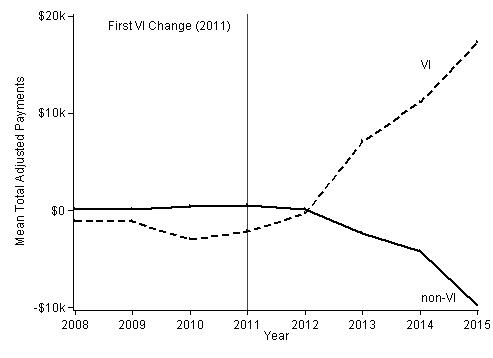
\includegraphics[height=2.5in,width=5in,keepaspectratio]{Summary_Pay3}
        \end{figure}
    }
\end{frame}


\section{Estimation of Match Values}
\begin{frame}{Specification}
    \only<1>{
    Two-step estimation strategy:
    \begin{enumerate}
        \item Estimate $y_{ijk} = \alpha_{i} + x_{i}\beta + \Gamma_{jk} + \epsilon_{ijk}$ at patient level (separately by year)
        \item Estimate $\hat{\Gamma}_{jkt} = \gamma_{j} + \gamma_{k} + \tau_{t} + z_{jkt}\delta + \eta_{jkt}$ with physician-hospital panel
    \end{enumerate}
    }
    \only<2>{
    \begin{equation*}
        y_{ijk} = \alpha_{i} + x_{i}\beta + \Gamma_{jk} + \epsilon_{ijk},
    \end{equation*}
    }
\end{frame}

\begin{frame}{Outcomes}
    \begin{equation*}
        \textcolor{red}{y_{ijk}} = \alpha_{i} + x_{i}\beta + \Gamma_{jk} + \epsilon_{ijk},
    \end{equation*}

    \begin{itemize}
        \item Total inpatient and outpatient Medicare payments
        \item Total inpatient and outpatient hospital costs (from cost-to-charge ratios)
        \item Total number of procedures
    \end{itemize}
\end{frame}


\begin{frame}{Independent Variables}
    \begin{equation*}
        y_{ijk} = \textcolor{red}{\alpha_{i}} + x_{i}\beta + \Gamma_{jk} + \epsilon_{ijk},
    \end{equation*}

    \begin{itemize}
        \item Quartiles of total prior Medicare payments and procedures
        \item Covers call payments/procedures (not just elective)
        \item Beneficiary-specific ranking of health care utilization up to time $t$
    \end{itemize}
\end{frame}

\begin{frame}{Independent Variables}
    \begin{equation*}
        y_{ijk} = \alpha_{i} + \textcolor{red}{x_{i}}\beta + \Gamma_{jk} + \epsilon_{ijk},
    \end{equation*}

    \begin{itemize}
        \item Age, gender, race
        \item Indicators for ICD9 diagnosis code groups (18 diagnosis groups per variable plus missing group)
    \end{itemize}
\end{frame}

\begin{frame}{Summary of Match Values}
    \only<1>{
        \metroset{block=fill}
        \begin{block}{1. Calculate Cost Differential}
            Apply minimum cost physician-hospital combination to all of physician $j$'s patients:
            \begin{align*}
                \Delta_{k} y_{ij} &= \hat{y}_{ijk} - \hat{y}_{ij\underbar{k}} \nonumber \\
                   &= \hat{\alpha}_{i} + x_{i}\hat{\beta} + \hat{\Gamma}_{jk} - \hat{\alpha}_{i} - x_{i}\hat{\beta} - \min \left\{\Gamma_{j1},...,\Gamma_{jK} \right\} \nonumber \\
                   &= \hat{\Gamma}_{jk} - \min \left\{\Gamma_{j1},...,\Gamma_{jK} \right\}.
            \end{align*}
        \end{block}
    }
    \only<2>{
        \metroset{block=fill}
        \begin{block}{2. Summarize}
            \begin{itemize}
                \item Total cost differential for each physician
                \item Limit to pairs with 5 or more procedures
                \item Limit to physicians with 2 or more hospitals in a year
                \item Present interquartile range and mean
            \end{itemize}
        \end{block}
    }

\end{frame}

\begin{frame}{Within-physician Variation in Payments}
    \only<1>{
        \begin{figure}
            \centering
            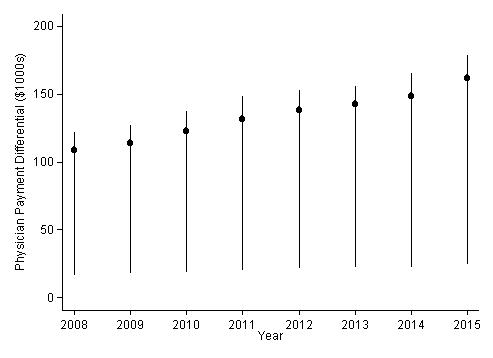
\includegraphics[height=2.5in,width=5in,keepaspectratio]{PhyPay_All_Graph}
        \end{figure}
    }
    \only<2>{
        \begin{figure}
            \centering
            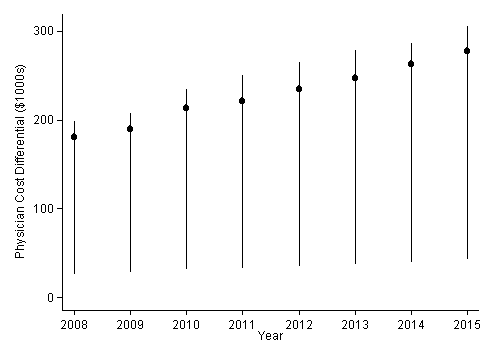
\includegraphics[height=2.5in,width=5in,keepaspectratio]{PhySave_All_Graph}
        \end{figure}
    }
\end{frame}


\section{Estimation of Hospital Influence}
\begin{frame}{Specification}
    \only<1>{
    Two-step estimation strategy:
    \begin{enumerate}
        \item Estimate $y_{ijk} = \alpha_{i} + x_{i}\beta + \Gamma_{jk} + \epsilon_{ijk}$ at patient level (separately by year)
        \item Estimate $\hat{\Gamma}_{jkt} = \gamma_{j} + \gamma_{k} + \tau_{t} + z_{jkt}\delta + \eta_{jkt}$ with physician-hospital panel
    \end{enumerate}
    }
    \only<2>{
    \begin{equation*}
        \hat{\Gamma}_{jkt} = \gamma_{j} + \gamma_{k} + \tau_{t} + z_{jkt}\delta + \eta_{jkt},
    \end{equation*}
    }
\end{frame}

\begin{frame}{Main Outcomes}
    \begin{equation*}
        \textcolor{red}{\hat{\Gamma}_{jkt}} = \gamma_{j} + \gamma_{k} + \tau_{t} + z_{jkt}\delta + \eta_{jkt},
    \end{equation*}

    \begin{table}[htb!]
    \centering
    \footnotesize
    \centerline{
    \begin{tabular}{l|rrrrr|r}
        & 2008  & 2012 & 2013 & 2014 & 2015 & Overall \\
        \hline
Total Payments &      6,367.7         &      7,301.9         &      7,644.3         &      8,021.9         &      8,234.8         &      7,238.4         \\
			   &    (5,454.5)         &    (6,385.4)         &    (6,562.7)         &    (6,658.9)         &    (6,822.7)         &    (6,219.2)         \onslide<2->{\\
Total Costs    &      8,384.5         &     10,168.8         &     10,600.5         &     11,029.3         &     11,466.5         &     9,851.9         \\
			   &    (6,822.1)         &   (8,165.1)         &   (8,410.1)         &   (8,754.5)         &   (8,935.2)         &   (7,994.5)         }\\
    \end{tabular}}
    \end{table}

\end{frame}


\begin{frame}{Independent Variables}
    \begin{equation*}
        \hat{\Gamma}_{jkt} = \gamma_{j} + \gamma_{k} + \tau_{t} + \textcolor{red}{z_{jkt}}\delta + \eta_{jkt},
    \end{equation*}

    \begin{table}[htb!]
    \centering
    \footnotesize
    \centerline{
    \begin{tabular}{l|rrrrr|r}
        & 2008  & 2012 & 2013 & 2014 & 2015 & Overall \\
        \hline
Integrated       &       0.129         &       0.205         &       0.232         &       0.254         &       0.327         &       0.196         \\
				 &     (0.336)         &     (0.404)         &     (0.422)         &     (0.435)         &     (0.469)         &     (0.397)        \onslide<2->{\\
Physician FTE       &       24.26         &       28.53         &       30.99         &       31.65         &       32.80         &       28.33         \\
					&     (99.19)         &     (109.6)         &     (120.1)         &     (119.7)         &     (118.9)         &     (110.6)         \onslide<3->{\\
Resident FTE        &       25.70         &       28.38         &       29.11         &       30.57         &       30.75         &       27.99         \\
					&     (108.1)         &     (120.3)         &     (121.4)         &     (125.6)         &     (127.3)         &     (117.5)         \onslide<4->{\\
Nurse FTE           &       341.1         &       365.0         &       367.5         &       383.9         &       400.1         &       363.9         \\
					&     (447.3)         &     (487.4)         &     (493.9)         &     (519.5)         &     (550.2)         &     (487.1)         \onslide<5->{\\
Other FTE           &       751.2         &       761.5         &       758.2         &       774.4         &       801.1         &       761.0         \\
					&     (978.4)         &    (1031.7)         &    (1073.9)         &    (1100.8)         &    (1155.5)         &    (1036.9)         \onslide<6->{\\
Beds (100s)         &       1.979         &       1.963         &       1.950         &       1.977         &       1.995         &       1.971         \\
					&     (2.160)         &     (2.141)         &     (2.135)         &     (2.177)         &     (2.231)         &     (2.153)         }}}}}\\
    \end{tabular}}
    \end{table}

\end{frame}

\begin{frame}{Independent Variables}
    \begin{equation*}
        \hat{\Gamma}_{jkt} = \gamma_{j} + \gamma_{k} + \tau_{t} + \textcolor{red}{z_{jkt}}\delta + \eta_{jkt},
    \end{equation*}

    \begin{table}[htb!]
    \centering
    \footnotesize
    \centerline{
    \begin{tabular}{l|rrrrr|r}
        & 2008  & 2012 & 2013 & 2014 & 2015 & Overall \\
        \hline
Practice Size &       13.81         &       17.39         &       17.40         &       17.96         &       18.65         &       16.21         \\
			  &     (32.27)         &     (30.83)         &     (29.42)         &     (28.68)         &     (28.43)         &     (30.24)         \onslide<2->{\\
Experience    &       22.55         &       23.00         &       23.93         &       23.65         &       24.76         &       23.16         \\
			  &     (6.498)         &     (6.704)         &     (6.953)         &     (6.901)         &     (6.999)         &     (6.748)         \onslide<3->{\\
\% Multi-Specialty &       0.249         &       0.248         &       0.266         &       0.284         &       0.344         &       0.264         \\
\% Surgery Center  &       0.452         &       0.500         &       0.506         &       0.507         &       0.452         &       0.479         }}\\
    \end{tabular}}
    \end{table}

\end{frame}

\begin{frame}{Estimated Effects of Vertical Integration}
    \vspace{0.75in}
    \begin{table}[htb!]
    \centering
    \centerline{
    \begin{tabular}{l|rr}
        Outcome & Estimate & St. Error \\
        \hline\hline \onslide<2->{\vspace{-.1in}\\
        Total Medicare Payments & 75.121** & (30.902)  \onslide<3->{\\
        Total Hospital Costs & 132.466***  & (42.026) \onslide<4->{\\
        Total Procedures   &   0.015***  &  (0.004) }}}\\
        \hline
        \multicolumn{3}{l}{\footnotesize * p-value $<$0.1, ** p-value $<$0.05, *** p-value $<$0.01}
    \end{tabular}}
    \end{table}
\end{frame}


\begin{frame}{Threats to Identification and Interpretation}
    Estimator is effectively a two-way fixed effects DD with time varying treatment
    \only<2>{
        \metroset{block=fill}
        \begin{block}{Potential Problems}
            \begin{enumerate}
                \item Vertical integration due to time-varying unobservables \& outcomes (standard DD concern)
                \item Weighted average of all 2$\times$2 DD estimates, with some potentially negative weights
            \end{enumerate}
        \end{block}
    }
\end{frame}

\begin{frame}{Event Study: Total Medicare Payments}
    \begin{figure}
        \centering
        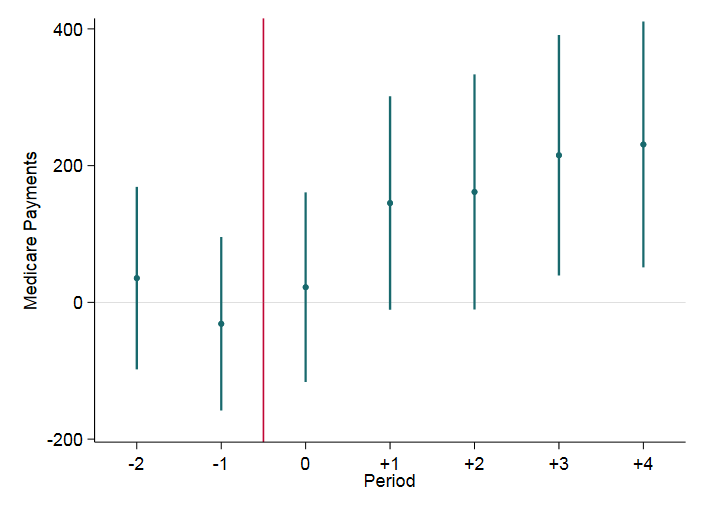
\includegraphics[height=2.5in,width=5in,keepaspectratio]{EventPay_All_2011}
    \end{figure}
\end{frame}

\begin{frame}{Event Study: Total Hospital (IP \& OP) Costs}
    \begin{figure}
        \centering
        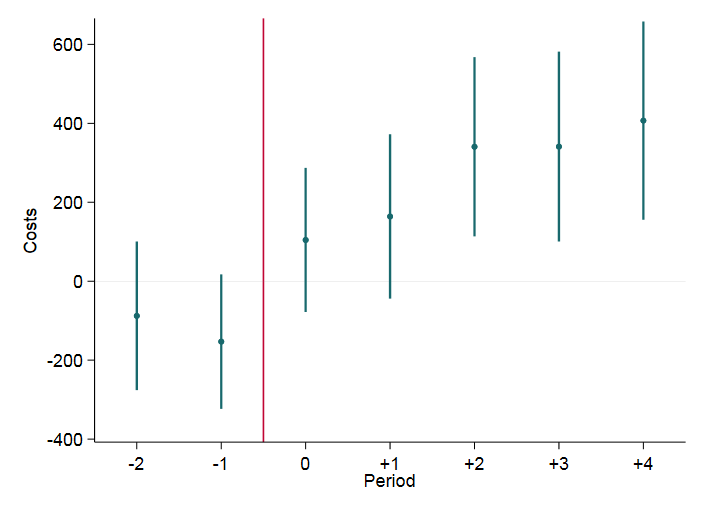
\includegraphics[height=2.5in,width=5in,keepaspectratio]{EventCharge_All_2011}
    \end{figure}
\end{frame}

\begin{frame}{Takeaways}
    \begin{itemize}
        \item Increase in payments and costs
        \item Evidence consistent with common trends assumption for total payments and costs
        \item Concerns about limited pre-period data
    \end{itemize}
\end{frame}


\begin{frame}{Endogeneity of physician-hospital integration}
    \label{ivs}
    \only<1>{
        Integration could be driven by:
        \begin{itemize}
            \item Unobserved, time-varying practice characteristics
            \item Existing costs and treatment patterns
        \end{itemize}
    }
    \only<2>{
        \metroset{block=fill}
        \begin{block}{1. Set of possible physician-hospital pairs}
            Form set of all hospitals where physician operates from 2008-2015
        \end{block}
    }
    \only<3>{
        \metroset{block=fill}
        \begin{block}{2. Estimate probability of integration}
            \begin{equation*}
                \text{Pr}\left(I_{jk}=1\right) = \frac{\text{exp}\left(\lambda z_{jk}\right)}{1+\text{exp}\left(\lambda z_{jk}\right)}
            \end{equation*}
            \vspace{-.3in}
            \begin{itemize}
                \item Hospital and practice characteristics
                \item Average differential distance (relative to nearest hospital in patient choice set)
                \item Differential distance interacted with hospital and practice characteristics
            \end{itemize}
        \end{block}
    }
    \only<4>{
        \metroset{block=fill}
        \begin{block}{2. Estimate probability of integration}
            \begin{equation*}
                \hat{\text{Pr}}\left(I_{jk}=1\right) = \frac{\text{exp}\left(\hat{\lambda} z_{jk}\right)}{1+\text{exp}\left(\hat{\lambda} z_{jk}\right)}
            \end{equation*}
            \noindent Intuition: Physicians less likely to seek/allow acquisition if patients live further away
        \end{block}
    }
    \only<5>{
        \metroset{block=fill}
        \begin{block}{2. Estimate probability of integration}
            \begin{equation*}
                \hat{\text{Pr}}\left(I_{jk}=1\right) = \frac{\text{exp}\left(\hat{\lambda} z_{jk}\right)}{1+\text{exp}\left(\hat{\lambda} z_{jk}\right)}
            \end{equation*}
            \noindent Intuition: Physicians less likely to seek/allow acquisition if patients live further away
        \end{block}
        \begin{equation*}
            \hat{\Gamma}_{jkt} = \gamma_{j} + \gamma_{k} + \tau_{t} + \underbrace{I_{jkt}}_{\mathclap{\hat{I}_{jkt}=\hat{\text{Pr}}(I_{jkt}=1)}} \delta_{1}  + \tilde{z}_{jkt}\delta_{2} + \eta_{jkt},
        \end{equation*}
    }
\end{frame}

\begin{frame}{IV Results: Aggregate Outcomes}
    \vspace{0.75in}
    \begin{table}[htb!]
    \centering
    \centerline{
    \begin{tabular}{l|rr}
        Outcome & Estimate & St. Error \\
        \hline\hline \onslide<2->{\vspace{-.1in}\\
        Total Medicare Payments & 870.4** & (340.41)  \onslide<3->{\\
        Total Hospital Costs & 2,546***  & (454.70) \onslide<4->{\\
        Total Procedures & 0.271*** & (0.042) }}}\\
        \hline
        \multicolumn{3}{l}{\footnotesize * p-value $<$0.1, ** p-value $<$0.05, *** p-value $<$0.01}
    \end{tabular}}
    \end{table}
\end{frame}

\section{Heterogeneities in Effects}
\begin{frame}{Unconditional Quantile Results: Payments}
    \begin{figure}
        \centering
        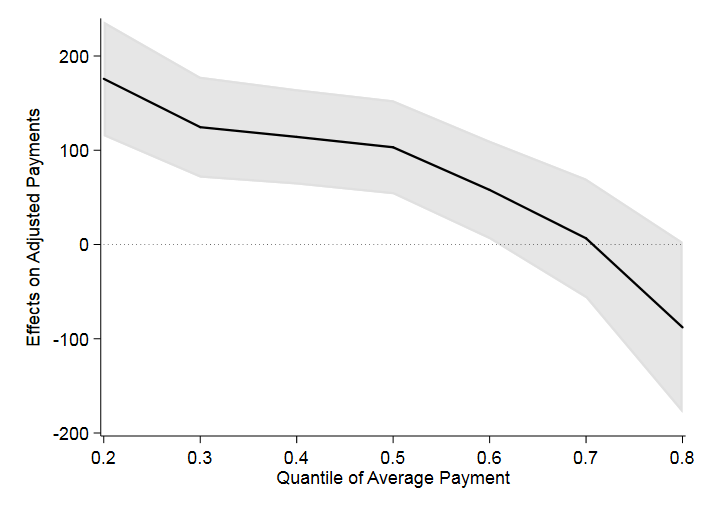
\includegraphics[height=2.5in,width=5in,keepaspectratio]{QReg_Payment}
    \end{figure}
\end{frame}

\begin{frame}{Unconditional Quantile Results: Hospital Costs}
    \begin{figure}
        \centering
        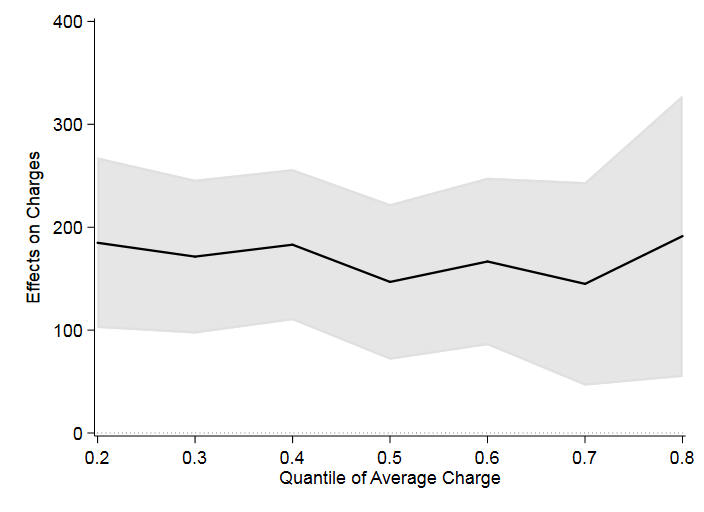
\includegraphics[height=2.5in,width=5in,keepaspectratio]{QReg_Charge}
    \end{figure}
\end{frame}

\begin{frame}{Unconditional Quantile Results: Procedures}
    \begin{figure}
        \centering
        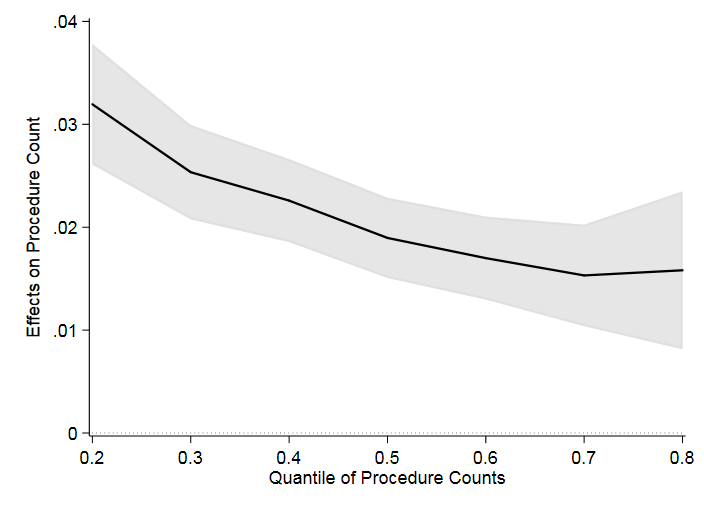
\includegraphics[height=2.5in,width=5in,keepaspectratio]{QReg_Procs}
    \end{figure}
\end{frame}

\section{Treatment Intensity vs Reallocation}

\begin{frame}{Want to isolate treatment intensity effect}
    \begin{enumerate}
        \item Focus on patients with no change in physician/hospital pairs over time
        \item Examine outcomes within an inpatient stay
    \end{enumerate}
\end{frame}

\begin{frame}{Aggregate Outcomes without Reallocation}
    \vspace{0.75in}
    \begin{table}[htb!]
    \centering
    \centerline{
    \begin{tabular}{l|rr}
        Outcome & Estimate & St. Error \\
        \hline\hline \onslide<2->{\vspace{-.1in}\\
        Total Medicare Payments & 63.291** & (30.853)  \onslide<3->{\\
        Total Hospital Costs & 124.830***  & (42.073) \onslide<4->{\\
        Total Procedures & 0.014** & (0.004) }}}\\
        \hline
        \multicolumn{3}{l}{\footnotesize * p-value $<$0.1, ** p-value $<$0.05, *** p-value $<$0.01}
    \end{tabular}}
    \end{table}
\end{frame}

\begin{frame}{Effects on Components of Inpatient Stay}
    \vspace{0.5in}
    \begin{table}[htb!]
    \centering
    \centerline{
    \begin{tabular}{l|rr}
        Outcome & Estimate & St. Error \\
        \hline\hline
        Charges for: & & \\
        \hspace{.1in} Total Inpatient & 165.441*** & (50.165) \\
        \hspace{.1in} Medical Supplies & 40.413 & (30.299) \\
        \hspace{.1in} Operating Room & -1.780 & (22.996) \\
        \hspace{.1in} Anesthesia & 6.504 & (4.970) \\
        \hspace{.1in} Labs & 14.006 & (8.782) \\
        \hspace{.1in} Radiology & -2.366 & (5.971) \\
        \hspace{.1in} MRI & -0.073 & (1.386) \\
        \hline
        \multicolumn{3}{l}{\footnotesize * p-value $<$0.1, ** p-value $<$0.05, *** p-value $<$0.01}
    \end{tabular}}
    \end{table}
\end{frame}

\begin{frame}{Effects on Components of Inpatient Stay}
    \vspace{0.5in}
    \begin{table}[htb!]
    \centering
    \centerline{
    \begin{tabular}{l|rr}
        Outcome & Estimate & St. Error \\
        \hline\hline
        Counts of: & & \\
        \hspace{.1in} ICU Days  & 0.022* & (0.013) \\
        \hspace{.1in} Procedures  & 0.030*** & (0.009) \\
        \hline
        \multicolumn{3}{l}{\footnotesize * p-value $<$0.1, ** p-value $<$0.05, *** p-value $<$0.01}
    \end{tabular}}
    \end{table}
\end{frame}



\section{Allocation of Procedures and Patients}
\begin{frame}{Other Effects}
    Other ways integration posited to affect physician behavior:
    \begin{itemize}
        \item More procedures overall (not per patient)
        \item Reallocating procedures from other hospitals
        \item Reallocating procedures across inpatient and outpatient settings
        \item Changing patient profile
    \end{itemize}
\end{frame}

\begin{frame}{Results on Other Outcomes}
    \vspace{.15in}
    \begin{table}[htb!]
    \centering
    \centerline{
    \begin{tabular}{l|rr}
        \hline
        Outcome & Estimate & St. Error \\
        \hline\hline \onslide<2->{\vspace{-.1in}\\
        Physician's inpatient share & 0.083*** & (0.003) \onslide<3->{\\
        Physician's outpatient share & 0.063***  & (0.003) \onslide<4->{\\
        Total patients & 7.304*** & (0.500) \onslide<5->{\\
        Inpatient procedures & 1.124*** & (0.161) \onslide<6->{\\
        Outpatient procedures & 10.375*** & (1.001) \onslide<7->{\\
        Patient Claims     & 0.013  & (0.058)  \onslide<8->{\\
        Patient Payments   & -156.713 & (136.992)  }}}}}}}\\
        \hline
        \multicolumn{3}{l}{\footnotesize * p-value $<$0.1, ** p-value $<$0.05, *** p-value $<$0.01}
    \end{tabular}}
    \end{table}
\end{frame}

\begin{frame}{Summary of Results}
    \only<1>{
        \metroset{block=fill}
        \begin{block}{Overall Results}
            \begin{itemize}
                \item Increase in Medicare payments (\$75-\$200) and hospital costs (\$130-\$350)
                \item Extrapolates to between \$52mm and \$140mm in additional Medicare payments per year
                \item 4-10\% of within-physician variation explained by vertical integration
            \end{itemize}
        \end{block}
    }

    \only<2>{
        \metroset{block=fill}
        \begin{block}{Sensitivity}
           \begin{itemize}
                \item Event study consistent with common pre-trends but limited pre-period data
                \item IV results suggest conservative estimates
                \item No improvement in quality (mortality)
                \item As falsification test, no effects on payments or DRG weights per inpatient stay
            \end{itemize}
        \end{block}
    }
\end{frame}

\section*{Thank You}


\end{document}






